\subsection{Constraints on \tesss Observing}
\label{sec:constraints_on_pointings}

When considering possible schedules for telescope pointings, the main
constraint is that the cameras must be directed approximately opposite
the Sun.  Specifically, the center of the combined fields-of-view is
ideally pointed within 15$^\circ$ in ecliptic longitude of the antisolar 
direction, and no more than 30$^\circ$ away.
%\todo[inline]{Roland: are these numbers still good? are they imposed by the sunshade? or solar panels? Some comment appreciated.} 
This enables the solar panels (which are free to rotate
about the $+Y$ axis in Fig.~\ref{fig:spacecraft_angles}) to collect
sufficient sunlight to power the spacecraft.
To a lesser extent, it is also necessary for the sunshade and 
spacecraft to block solar photons.
Given the spacecraft's orbit~\citep{gangestad_high_2013},
this means that \tess should advance $\sim$$28^\circ$ east in ecliptic
longitude every lunar month, as it does during the Primary Mission.
Focusing on a fixed field for say, 3 spacecraft orbits ($\approx$42
days), would be in tension with this requirement.  In practice,
another technical restriction is whether the Earth or Moon passes
through \tesss camera fields during a proposed pointing (see
Sec.~\ref{sec:earth_moon_crossings}).

In addition, the spacecraft has finite fuel reserves for necessary maneuvers.
These are expected to last at least 10 years [G. Ricker, priv. comm.]. We 
consequently do not consider this as a constraint on the three-year time 
horizon that is the focus of this study.

\begin{figure}[!b]
	\centering
	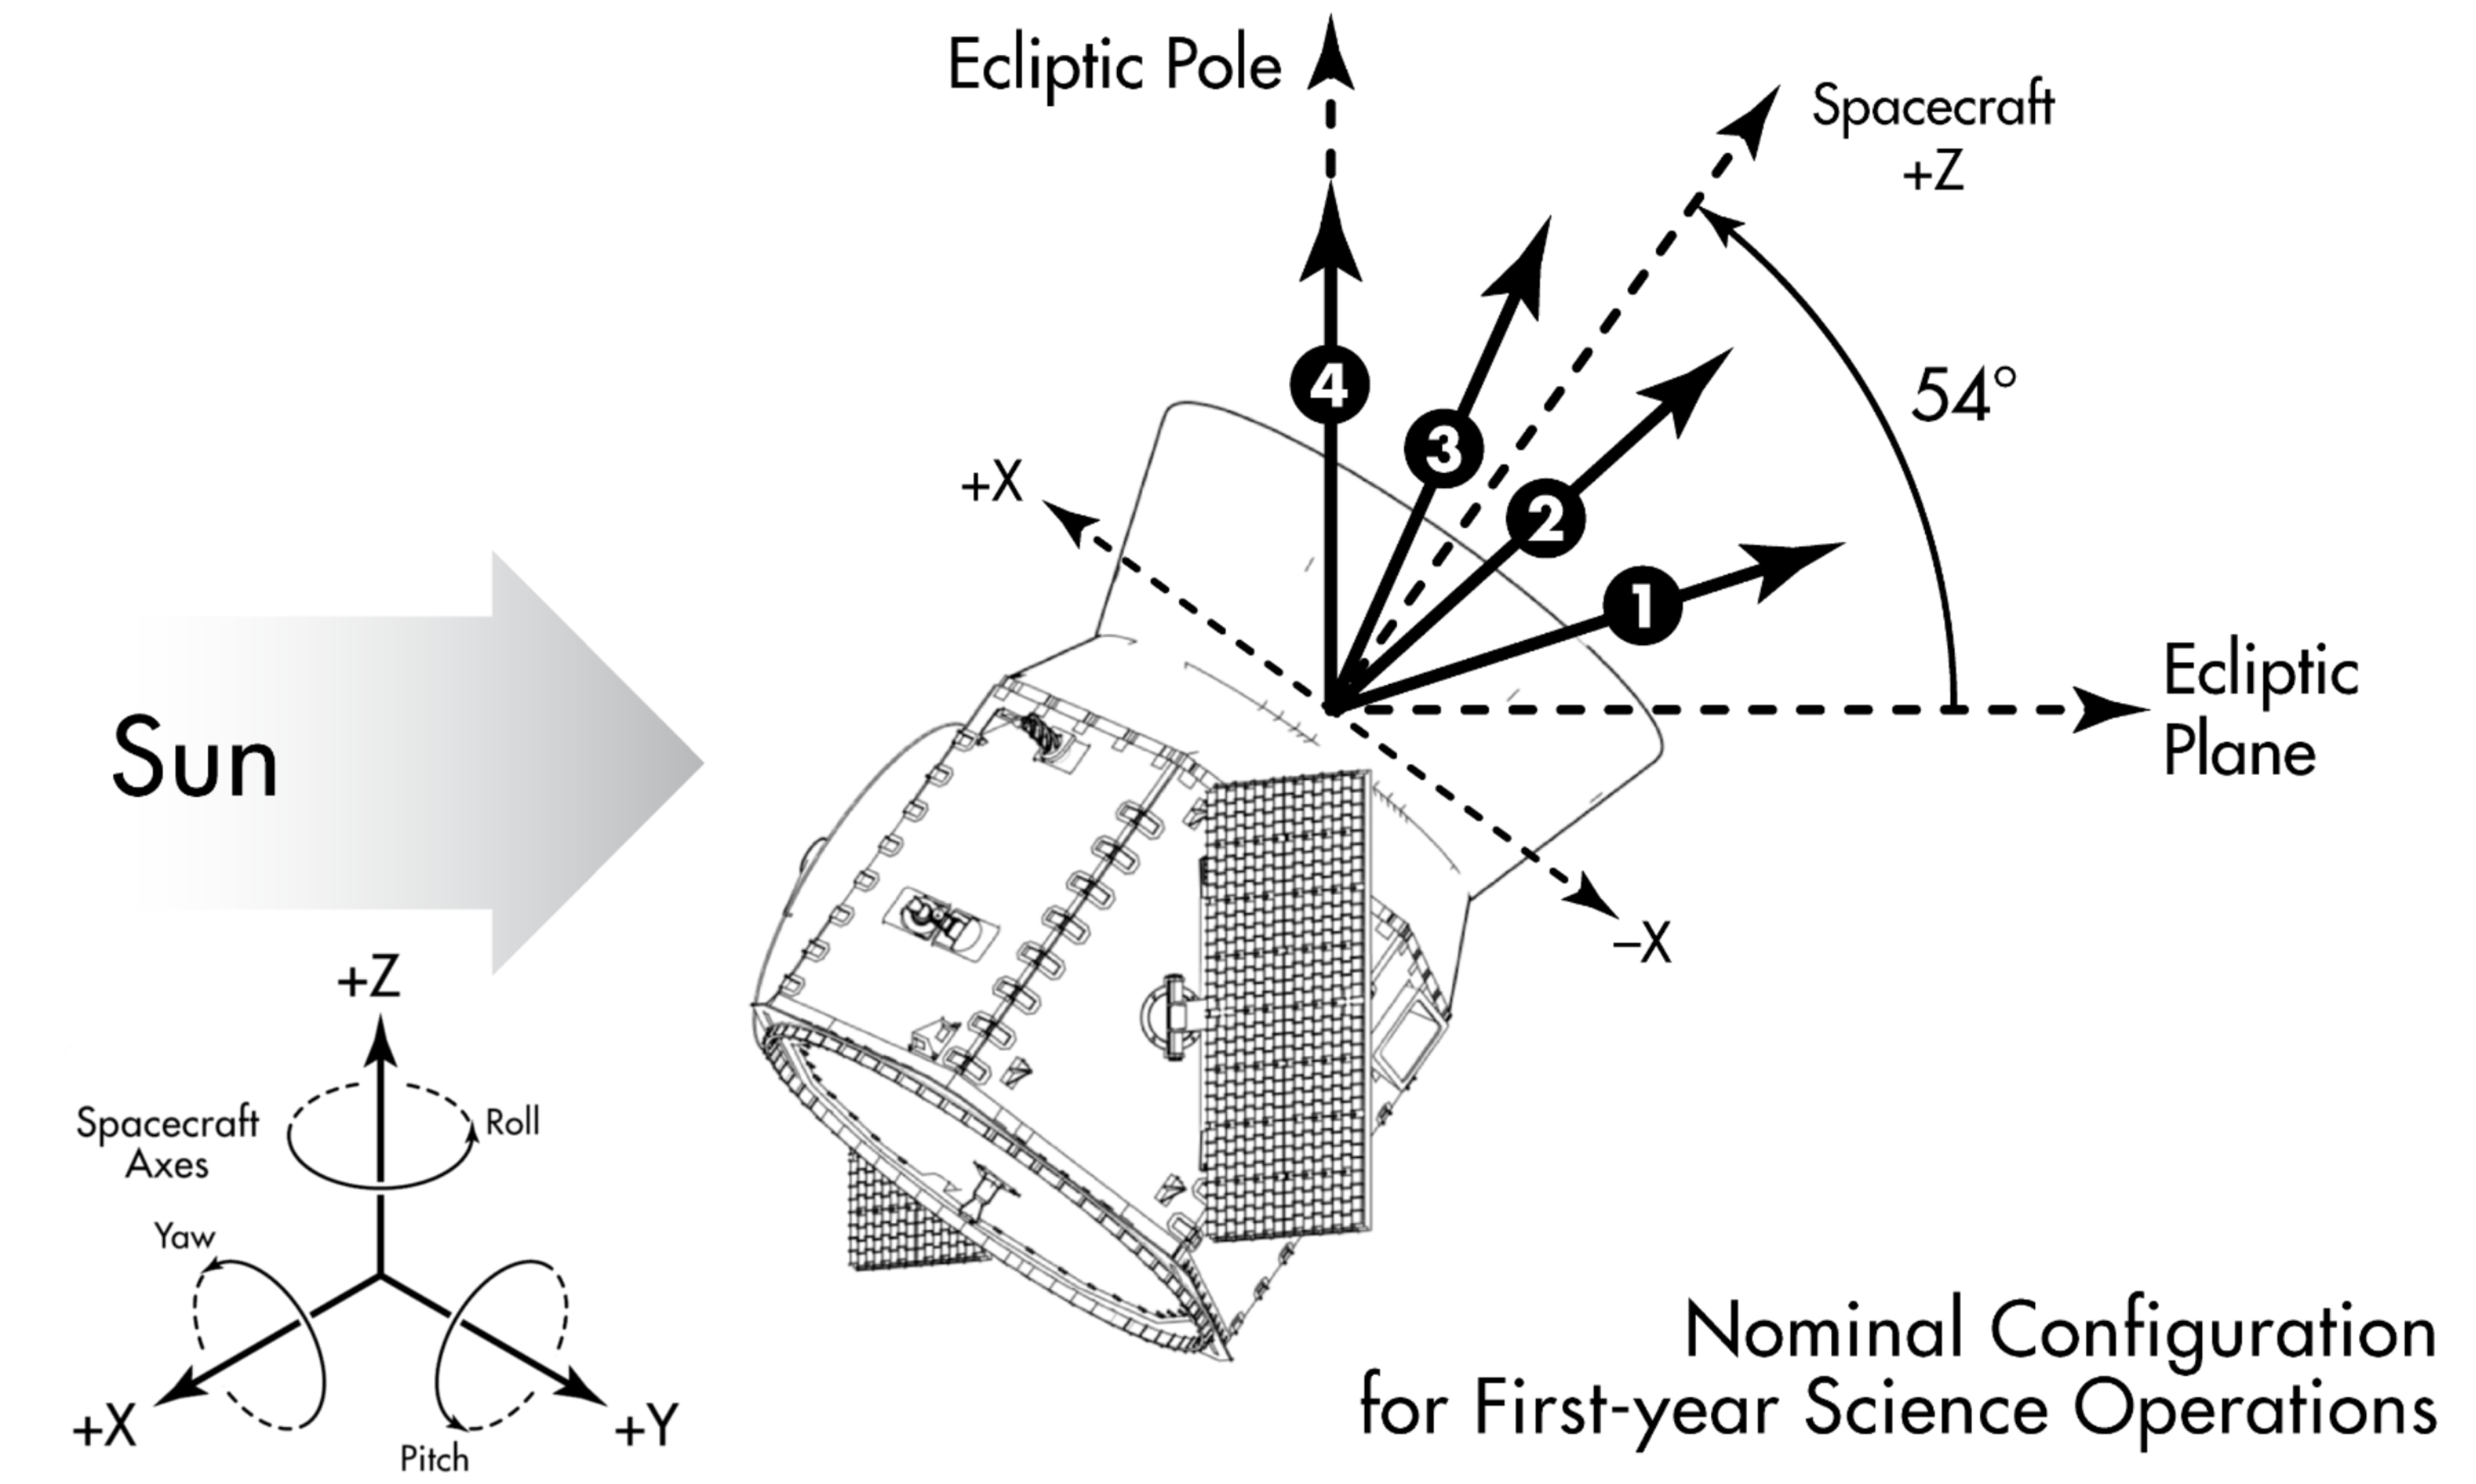
\includegraphics{figures/spacecraft_angles.pdf}
	\caption{The spacecraft must point so that incident sunlight is collected 
		by the solar panels, and not the cameras. \tesss solar panels pitch 
		about the $+Y$ axis. (Adapted from Orbital ATK design document) }
	\label{fig:spacecraft_angles}
\end{figure}
